\section{Abstract}\label{abstract}

Speech-science experiments often require synthetic stimuli that are
natural enough for repeated listening, but also explicitly controllable
along phonetically meaningful dimensions such as fundamental frequency,
formant frequency, spectral tilt, intensity, and voice quality. Modern
neural vocoders provide high perceptual quality, but their data
requirements and latent acoustic representations can make them difficult
to use in small-data phonetic studies. Classical formant synthesis
provides interpretability and control, but often lacks the naturalness
required for ecological experimental stimuli. This paper presents
ARIA-NSF, a differentiable Klatt-style neural source-filter synthesizer
designed for small-data, single-speaker phonetic stimulus generation.
The model combines an analytic glottal excitation controlled by \(F_0\)
and \(R_d\), a learned noise component, and a vocal-tract cascade that
combines deterministic formant/all-pole sections with learned biquad
residual sections. In the current configuration, the vocal-tract cascade
contains three deterministic biquad sections and eight learned biquads,
yielding an LPC-equivalent order of \(2(3+8)=22\). Rather than proposing
a general-purpose neural vocoder, ARIA-NSF targets a narrower
experimental setting: controllable copy synthesis and acoustic
manipulation from laboratory-scale speech recordings. We describe the
architecture, the pilot Mandarin corpus, and a concrete evaluation plan
covering acoustic error, parameter disentanglement, baseline comparison,
and perceptual validation.

\textbf{Keywords:} neural source-filter model; formant synthesis;
differentiable DSP; phonetic stimulus generation; small-data speech
synthesis; voice quality

\section{1. Introduction}\label{introduction}

Controlled speech synthesis occupies an unusual position between speech
technology and phonetic science. In text-to-speech and neural vocoding,
the primary goal is often perceptual naturalness, speaker similarity, or
large-scale generalization. In phonetic and psycholinguistic
experiments, however, the research goal is frequently different: the
stimulus must be natural enough to be listened to repeatedly, but the
experimental manipulation must also be interpretable, precise, and
preferably low-dimensional. A phonetician may need to shift \(F_0\) to
create a tone or intonation continuum, move \(F_1\) and \(F_2\)
independently to construct a vowel continuum, or alter source-related
parameters to probe breathy, creaky, or pressed voice quality. A system
that produces plausible audio but hides these variables inside a
high-dimensional latent representation is therefore not always suitable
for experimental work.

This requirement is especially challenging in typical speech-science
settings. Unlike modern speech-generation pipelines, which may rely on
many hours or thousands of hours of training data, experimental
materials are often collected for a specific study. A dataset may
contain only 5--60 minutes of speech from one speaker, recorded under a
controlled design for a particular phenomenon such as tone sandhi,
categorical perception, prosodic prominence, vowel normalization, or
phonation type. Such datasets are valuable precisely because they are
tailored to a hypothesis, but they are usually too small to support
large generic neural vocoders without overfitting, artifacts, or loss of
controllability.

Classical source-filter theory (\citeproc{ref-fant1960acoustic}{Fant
1960}) and formant synthesis (\citeproc{ref-klatt1980software}{Klatt
1980}) offer the right conceptual primitives: a source, a vocal-tract
filter, and interpretable acoustic controls. Tools such as Praat
(\citeproc{ref-boersma2001praat}{Boersma 2001}) remain central in
phonetics because they support analysis and manipulation in terms that
phoneticians understand. Yet purely classical synthesis can sound
unnatural, especially when used to create full experimental stimuli
rather than isolated demonstrations. Conversely, modern neural vocoders
and neural source-filter models can generate high-quality waveforms
(\citeproc{ref-wang2020nsf}{Wang et al. 2020}), but their control
variables are often less directly aligned with experimental
manipulations.

This paper presents ARIA-NSF, a small-data differentiable Klatt-style
neural source-filter synthesizer. The central design hypothesis is that
phonetic stimulus generation benefits from a hybrid allocation of
responsibility: parameters that are experimentally meaningful and
acoustically well-understood should remain analytic or deterministic,
while the residual aspects of timbre and spectral detail can be learned
from data. In the current implementation, \(F_0\), \(F_1\), \(F_2\),
bandwidths, gain, spectral tilt, and glottal-source parameters are
exposed as controllable variables. A small neural model predicts or
refines the remaining control streams needed for copy synthesis.

The intended contribution is not a universal TTS system. Instead,
ARIA-NSF targets a narrower but common research use case: creating
high-quality, interpretable speech stimuli from a small, single-speaker
corpus. The paper makes three contributions:

\begin{enumerate}
\def\labelenumi{\arabic{enumi}.}
\tightlist
\item
  It formulates the requirements of neural speech synthesis for phonetic
  stimulus generation as a small-data, high-control source-filter
  problem.
\item
  It introduces a differentiable Klatt-style architecture that combines
  an analytic glottal source, shaped noise, deterministic formant
  sections, and learned residual biquads.
\item
  It defines a pilot Mandarin evaluation protocol for measuring
  copy-synthesis quality, manipulation reliability, and unwanted
  acoustic coupling.
\end{enumerate}

\section{2. Related Work}\label{related-work}

\subsection{2.1 Classical Formant Synthesis and Phonetic
Manipulation}\label{classical-formant-synthesis-and-phonetic-manipulation}

The source-filter model of speech production provides a compact account
of speech as the interaction between a laryngeal source and a
vocal-tract filter (\citeproc{ref-fant1960acoustic}{Fant 1960}). Klatt's
cascade/parallel formant synthesizer
(\citeproc{ref-klatt1980software}{Klatt 1980}) made this account
operational by exposing parameters such as formant frequencies,
bandwidths, voicing amplitude, aspiration, frication, and spectral tilt.
For phonetic experiments, this level of control remains attractive
because it allows a researcher to manipulate one acoustic dimension
while holding others approximately constant.

The limitation is perceptual quality. Even when a classical formant
synthesizer accurately implements an acoustic hypothesis, the resulting
stimulus may sound synthetic in ways that affect listener behavior. This
matters because perceptual experiments are not only tests of acoustic
discriminability; they are also embedded in listeners' expectations
about natural speech. A stimulus continuum with audible artifacts may
therefore confound the intended manipulation.

Praat (\citeproc{ref-boersma2001praat}{Boersma 2001}) and LPC-based copy
synthesis remain widely used because they allow practical analysis and
manipulation of pitch and formant-related properties. However, inverse
filtering and source-filter separation are imperfect. If formant
information remains in the residual excitation, formant manipulation can
introduce artifacts or unintended acoustic coupling.

\subsection{2.2 Neural Source-Filter and Differentiable DSP
Models}\label{neural-source-filter-and-differentiable-dsp-models}

Neural source-filter models reintroduced speech-production structure
into neural waveform generation. Wang et al.
(\citeproc{ref-wang2020nsf}{2020}) proposed an NSF framework in which a
source module generates an excitation signal, a neural filter module
transforms it into a waveform, and a condition module preprocesses
acoustic features. This design preserves explicit \(F_0\)-driven
excitation while avoiding autoregressive generation.

Differentiable digital signal processing (DDSP) similarly argues that
neural audio models can benefit from embedding known signal-processing
operators inside trainable systems (\citeproc{ref-engel2020ddsp}{Engel
et al. 2020}). Rather than learning the entire waveform generator as an
unconstrained network, DDSP systems can learn control parameters for
interpretable modules such as oscillators, filters, and reverberation.
This is especially relevant for small-data settings, where inductive
bias can reduce the amount of data required to learn a usable
synthesizer.

GOLF (\citeproc{ref-yu2024golf}{Yu and Fazekas 2024}) is a particularly
close reference point. It uses glottal-flow wavetables as the harmonic
source and LPC filters to model the vocal tract, achieving a compact and
efficient singing voice synthesizer. GOLF shows that voice-production
constraints can be integrated into differentiable synthesis while
maintaining competitive quality and efficiency. ARIA-NSF follows the
same general philosophy but targets speech-science stimulus generation
rather than singing voice synthesis, and gives priority to explicit
manipulation of \(F_0\), \(F_1/F_2\), and source-shape parameters.

HiFi-Glot (\citeproc{ref-gu2026hifiglot}{Gu et al. 2026}) addresses a
related problem from the direction of high-fidelity neural formant
synthesis. It combines neural excitation with differentiable
resonant/all-pole filters to provide explicit formant control at high
perceptual quality. Compared with such full-band, large-capacity
systems, ARIA-NSF is deliberately smaller and more specialized. It
sacrifices some generality in favor of small-data trainability, explicit
experimental controls, and a structure that remains close to traditional
formant synthesis.

\subsection{2.3 Source-Filter
Positioning}\label{source-filter-positioning}

The source-filter taxonomy used in uSFGAN
(\citeproc{ref-yoneyama2021usfgan}{Yoneyama et al. 2021}) is useful for
locating ARIA-NSF among conventional vocoders, neural source-filter
models, and fully neural waveform generators. In that taxonomy,
excitation generation and resonance filtering can each be implemented as
deterministic/parametric modules, neural modules, or a unified neural
waveform generator. Figure 1 adapts this view and places ARIA-NSF as a
dual-hybrid source-filter model.

\begin{figure}
\centering
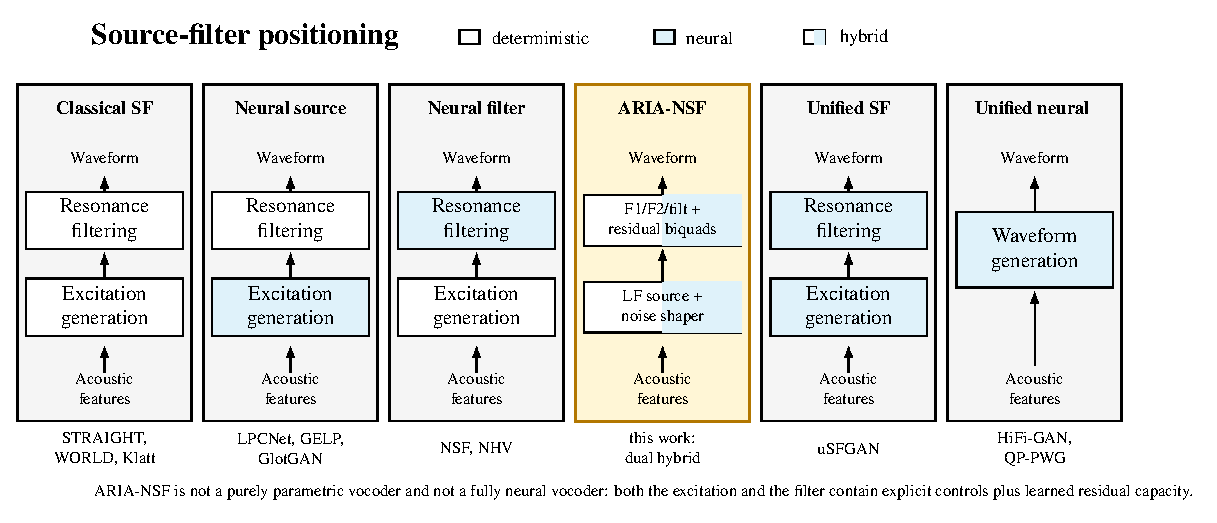
\includegraphics[width=1\linewidth,height=\textheight,keepaspectratio,alt={Positioning of ARIA-NSF within source-filter vocoder architectures. The diagram is adapted from the source-filter taxonomy in uSFGAN (Yoneyama et al. 2021), but adds the ARIA-NSF column to emphasize that both excitation generation and resonance filtering are hybrid rather than purely deterministic or purely neural.}]{figures/aria_source_filter_positioning_tikz.pdf}
\caption{Positioning of ARIA-NSF within source-filter vocoder
architectures. The diagram is adapted from the source-filter taxonomy in
uSFGAN (\citeproc{ref-yoneyama2021usfgan}{Yoneyama et al. 2021}), but
adds the ARIA-NSF column to emphasize that both excitation generation
and resonance filtering are hybrid rather than purely deterministic or
purely neural.}
\end{figure}

ARIA-NSF is therefore better described as structurally hybrid than as a
literal 50/50 split between deterministic and neural components. On the
excitation side, the periodic glottal source is generated
deterministically from \(F_0\) and \(R_d\), while the aperiodic/noise
component is learned or conditioned. On the filter side, the
experimentally important vocal-tract controls remain deterministic and
interpretable, while learned residual biquads supply speaker-specific
spectral detail. The model thus splits responsibility in both places:
explicit DSP handles the variables that should remain editable, and
neural residual capacity handles details that are difficult to specify
by hand.

\section{3. Design Requirements}\label{design-requirements}

ARIA-NSF is designed around five requirements that are common in
phonetic stimulus generation but less central in general-purpose neural
vocoding.

\textbf{R1. Small-data trainability.} The system should be usable with
5--60 minutes of single-speaker recordings, because phonetic corpora are
often collected for a narrow experimental question rather than for
large-scale speech generation.

\textbf{R2. Explicit intervention variables.} Experimental variables
such as \(F_0\), \(F_1/F_2\), bandwidth, gain, spectral tilt, and
\(R_d\) should remain directly editable. They should not be recoverable
only as post-hoc measurements from a generated waveform.

\textbf{R3. Low cross-parameter coupling.} Manipulating one dimension
should minimally disturb others. For example, an \(F_1\) manipulation
should not substantially alter \(F_0\), energy, or source-shape cues.

\textbf{R4. Residual expressivity.} Purely analytic formant synthesis
may not capture enough speaker-specific spectral detail for
natural-sounding stimuli. The architecture therefore needs limited
learned capacity, but this capacity must be constrained enough that it
does not erase interpretability.

\textbf{R5. Laboratory accessibility.} Training should be feasible on
consumer or modest institutional GPUs. This requirement is practical
rather than theoretical, but it is important for speech-science
laboratories without sustained access to large compute clusters.

These requirements motivate a dual-hybrid source-filter design:
deterministic components implement the experimental variables, while
learned residual components model aspects of both the excitation and the
filter that are difficult to specify analytically.

\section{4. Model}\label{model}

Figure 2 gives a schematic overview of the current ARIA-NSF pipeline.
The architecture operates at two rates. Frame-rate acoustic controls are
predicted, extracted, or specified by the user; these controls are then
upsampled to the audio sample rate for differentiable waveform
synthesis.

\begin{figure}
\centering
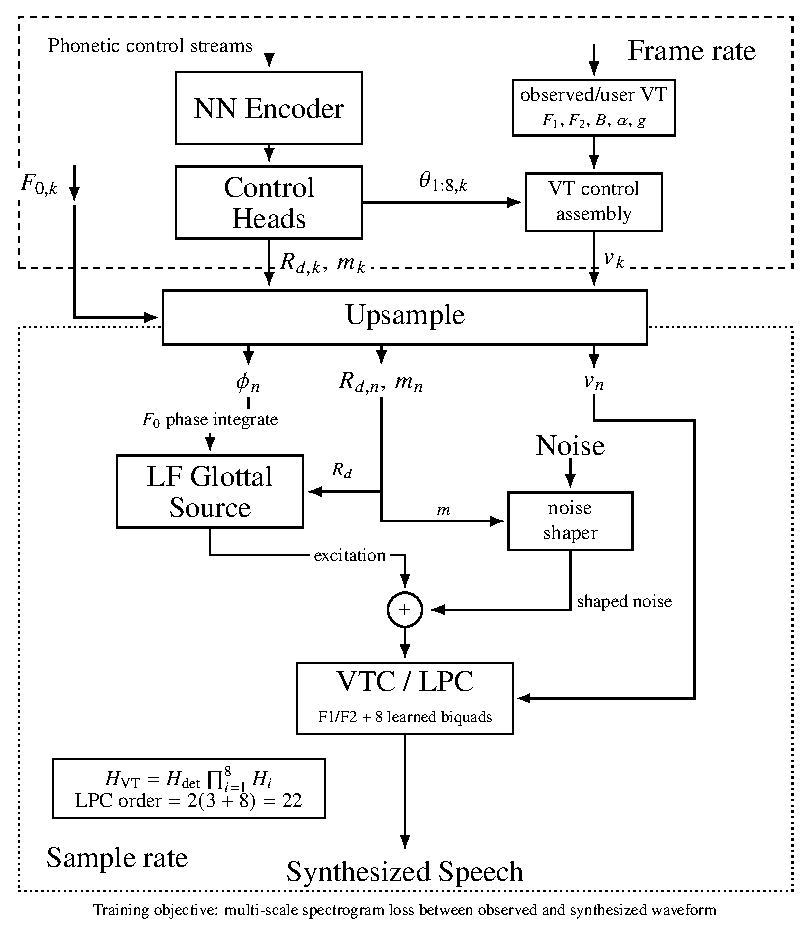
\includegraphics[width=0.8\linewidth,height=\textheight,keepaspectratio,alt={Current ARIA-NSF source-filter diagram. The glottal excitation and shaped noise are summed before passing through the vocal-tract cascade / LPC filter.}]{figures/aria_golf_f024_formula_flow_tikz.pdf}
\caption{Current ARIA-NSF source-filter diagram. The glottal excitation
and shaped noise are summed before passing through the vocal-tract
cascade / LPC filter.}
\end{figure}

\subsection{4.1 Sample-Rate Excitation}\label{sample-rate-excitation}

Given sampling rate \(f_s\), the deterministic phase trajectory is
obtained by integrating the frame- or sample-rate \(F_0\) contour:

\[
\phi_n = \phi_{n-1} + 2\pi \frac{F_{0,n}}{f_s}.
\]

The voiced excitation is generated by an LF-style glottal source:

\[
e_n = g_{\mathrm{LF}}(\phi_n; R_{d,n}),
\]

where \(R_d\) controls the glottal pulse shape and is intended to
support continuous manipulation of phonation-related dimensions such as
pressed or breathy voice. This formulation follows the spirit of
LF-family source modeling (\citeproc{ref-fant1985lf}{Fant et al. 1985}),
but is used here as a differentiable component inside a neural
source-filter synthesizer rather than as a complete standalone voice
model.

A noise branch models turbulent or aperiodic energy. White noise
\(\epsilon_n\) is transformed by a learned or conditioned noise shaper:

\[
\eta_n = \mathcal{N}(\epsilon_n; m_n),
\]

where \(m_n\) denotes the sample-rate noise control stream. In contrast
to architectures that filter harmonic and noise components through
separate output paths, ARIA-NSF currently combines excitation and shaped
noise before the vocal-tract filter:

\[
u_n = e_n + \eta_n.
\]

This design choice follows the intended speech-production
interpretation: the periodic and aperiodic components form a source-like
excitation, which is then shaped by the vocal tract.

\subsection{4.2 Vocal-Tract Cascade}\label{vocal-tract-cascade}

The output waveform is generated by passing the combined excitation
through a time-varying vocal-tract cascade:

\[
y_n = H_{\mathrm{VT}}(z; v_n) u_n.
\]

The filter is factorized into deterministic, interpretable sections and
learned residual sections:

\[
H_{\mathrm{VT}}(z; v_n)
=
H_{\mathrm{det}}(z; F_{1,n}, F_{2,n}, B_{1,n}, B_{2,n}, \alpha_n, g_n)
\cdot
\prod_{i=1}^{8} H_i(z; \theta_{i,n}).
\]

Each biquad section can be written as an all-pole resonator:

\[
H_i(z; \theta_i)
=
\frac{G_i}{1+a_{i,1}z^{-1}+a_{i,2}z^{-2}}.
\]

In the current configuration, the deterministic component contains three
biquad sections and the neural residual component contains eight learned
biquads. The resulting LPC-equivalent order is:

\[
\mathrm{order} = 2(3+8)=22.
\]

This configuration is intended to make the first formant-related degrees
of freedom explicitly controllable while leaving enough residual
capacity to learn speaker-specific spectral detail that would be
difficult to hand-code.

\subsection{4.3 Training Objective}\label{training-objective}

The pilot implementation is trained as a copy-synthesis model using a
multi-scale spectral reconstruction objective:

\[
\mathcal{L}_{\mathrm{MSSTFT}}
=
\sum_{r\in\mathcal{R}}
\left(
\left\| |S_r(x)|-|S_r(y)| \right\|_1
+
\left\| \log(|S_r(x)|+\epsilon)-\log(|S_r(y)|+\epsilon) \right\|_1
\right),
\]

where \(x\) is the target waveform, \(y\) is the synthesized waveform,
and \(S_r\) is an STFT operator at resolution \(r\). This objective is
consistent with the spectral-loss tradition in DDSP and neural
source-filter work (\citeproc{ref-engel2020ddsp}{Engel et al. 2020};
\citeproc{ref-wang2020nsf}{Wang et al. 2020};
\citeproc{ref-yu2024golf}{Yu and Fazekas 2024}), while keeping the
training procedure lightweight.

\section{5. Pilot Corpus and Experimental
Conditions}\label{pilot-corpus-and-experimental-conditions}

The current pilot corpus consists of Mandarin monosyllabic word
recordings collected for phonetic research. The recording session
contains approximately 1,400 word tokens, with about 30 minutes of
effective usable audio after trimming and quality control. This corpus
is representative of a common phonetic-laboratory scenario: the material
is carefully designed for a linguistic question, but it is much smaller
than the datasets normally used to train high-capacity neural vocoders.

The pilot evaluation is organized around three operations:

\begin{enumerate}
\def\labelenumi{\arabic{enumi}.}
\tightlist
\item
  \textbf{Copy synthesis:} reconstructing held-out utterances from
  extracted or predicted acoustic controls.
\item
  \textbf{Pitch manipulation:} modifying \(F_0\) trajectories while
  preserving other source-filter properties.
\item
  \textbf{Vowel and source manipulation:} independently altering
  \(F_1/F_2\) and \(R_d\) to create continua relevant to vowel
  perception and voice-quality perception.
\end{enumerate}

The planned experimental conditions are summarized in Table 1. The
30-minute condition is treated as the primary pilot setting. The 5- and
10-minute conditions test whether the architecture remains useful when
the available speech material is closer to the lower bound of many
phonetic laboratory datasets.

Table 1. Planned pilot and ablation conditions.

{\def\LTcaptype{none} % do not increment counter
\begin{longtable}[]{@{}
  >{\raggedright\arraybackslash}p{(\linewidth - 4\tabcolsep) * \real{0.3000}}
  >{\raggedleft\arraybackslash}p{(\linewidth - 4\tabcolsep) * \real{0.4000}}
  >{\raggedright\arraybackslash}p{(\linewidth - 4\tabcolsep) * \real{0.3000}}@{}}
\toprule\noalign{}
\begin{minipage}[b]{\linewidth}\raggedright
Condition
\end{minipage} & \begin{minipage}[b]{\linewidth}\raggedleft
Training material
\end{minipage} & \begin{minipage}[b]{\linewidth}\raggedright
Purpose
\end{minipage} \\
\midrule\noalign{}
\endhead
\bottomrule\noalign{}
\endlastfoot
Full pilot & approximately 30 min & Main copy-synthesis and manipulation
condition \\
Reduced data & approximately 10 min & Small-data robustness check \\
Minimal data & approximately 5 min & Lower-bound feasibility check \\
Ablation: no learned biquads & approximately 30 min & Tests contribution
of residual spectral modeling \\
Ablation: deterministic formants disabled & approximately 30 min & Tests
whether explicit formant control is necessary \\
Ablation: no shaped noise & approximately 30 min & Tests contribution of
aperiodic excitation \\
\end{longtable}
}

Early listening during development suggests that the model can converge
on the 30-minute corpus and can still produce usable output under 5--10
minute training conditions. These observations motivate the evaluation
but should not be interpreted as final benchmark results.

The model is lightweight enough to train on a laptop-class RTX 4060 GPU.
On an A100-class server GPU, training time is typically on the order of
tens of minutes for the current single-speaker setting. This resource
profile is important for speech-science laboratories, where continuous
access to large-scale GPU clusters is often unrealistic.

\section{6. Evaluation Protocol}\label{evaluation-protocol}

A formal evaluation should measure both synthesis quality and
manipulation validity. For phonetic stimulus generation, these two
dimensions are equally important. A system that sounds natural but fails
to control the intended variable is not useful for controlled
experiments; likewise, a precisely controlled but unnatural stimulus may
not support ecologically valid listening behavior.

\subsection{6.1 Baselines and Ablations}\label{baselines-and-ablations}

The evaluation should compare ARIA-NSF against baselines that represent
both phonetic practice and neural synthesis practice:

Table 2. Proposed baselines and ablation systems.

{\def\LTcaptype{none} % do not increment counter
\begin{longtable}[]{@{}
  >{\raggedright\arraybackslash}p{(\linewidth - 2\tabcolsep) * \real{0.5000}}
  >{\raggedright\arraybackslash}p{(\linewidth - 2\tabcolsep) * \real{0.5000}}@{}}
\toprule\noalign{}
\begin{minipage}[b]{\linewidth}\raggedright
System
\end{minipage} & \begin{minipage}[b]{\linewidth}\raggedright
Role in evaluation
\end{minipage} \\
\midrule\noalign{}
\endhead
\bottomrule\noalign{}
\endlastfoot
Natural recording & Upper reference for perceptual quality \\
Praat / LPC copy synthesis & Conventional phonetic manipulation
baseline \\
DDSP harmonic-plus-noise & Differentiable synthesis baseline without
explicit vocal-tract cascade \\
HiFi-Glot-style source-filter model & Strong neural formant-synthesis
reference, where feasible \\
ARIA-NSF without learned biquads & Tests whether residual capacity
improves quality \\
ARIA-NSF without deterministic formant sections & Tests whether explicit
formant control is responsible for manipulation accuracy \\
ARIA-NSF without shaped noise & Tests whether aperiodic excitation
improves naturalness \\
\end{longtable}
}

\subsection{6.2 Acoustic Evaluation}\label{acoustic-evaluation}

For copy synthesis, standard reconstruction metrics can be reported,
including multi-scale STFT loss, mel-cepstral distortion, \(F_0\) error,
and spectral-envelope error. For manipulation tasks, the more important
metric is target-tracking error. For formants:

\[
E_{F_i}
=
\frac{1}{T}
\sum_t
\left|
\widehat{F_i}(y_t)-F_i^{\mathrm{target}}(t)
\right|,
\quad i\in\{1,2\}.
\]

The same logic can be applied to \(F_0\), intensity, spectral tilt, and
any estimated correlate of voice quality. To measure unwanted coupling,
one can compute a manipulation cross-effect matrix. For example, when
\(F_1\) is manipulated, the analysis should report not only the \(F_1\)
error but also the induced changes in \(F_0\), \(F_2\), energy, tilt,
and \(R_d\)-related measures.

For reporting, the most important outcome is not a single aggregate
score but a separation between quality, target accuracy, and side
effects:

{\def\LTcaptype{none} % do not increment counter
\begin{longtable}[]{@{}
  >{\raggedright\arraybackslash}p{(\linewidth - 4\tabcolsep) * \real{0.3333}}
  >{\raggedright\arraybackslash}p{(\linewidth - 4\tabcolsep) * \real{0.3333}}
  >{\raggedright\arraybackslash}p{(\linewidth - 4\tabcolsep) * \real{0.3333}}@{}}
\toprule\noalign{}
\begin{minipage}[b]{\linewidth}\raggedright
Dimension
\end{minipage} & \begin{minipage}[b]{\linewidth}\raggedright
Example metric
\end{minipage} & \begin{minipage}[b]{\linewidth}\raggedright
Interpretation
\end{minipage} \\
\midrule\noalign{}
\endhead
\bottomrule\noalign{}
\endlastfoot
Copy quality & MS-STFT, MCD, spectral-envelope error & How well the
model reconstructs held-out speech \\
Pitch control & \(F_0\) RMSE after manipulation & Whether deterministic
excitation tracks the target \\
Formant control & \(F_1/F_2\) target-tracking error & Whether
vowel-space manipulations are accurate \\
Source control & acoustic/perceptual correlate of \(R_d\) & Whether
source-shape manipulation is interpretable \\
Coupling & cross-effect matrix & Whether manipulating one parameter
disturbs others \\
Efficiency & training time, inference RTF, model size & Whether the
system is usable in laboratory settings \\
\end{longtable}
}

\subsection{6.3 Perceptual Evaluation}\label{perceptual-evaluation}

For copy synthesis, a MUSHRA-like or CMOS listening test can compare
ARIA-NSF with natural recordings, Praat/LPC copy synthesis, and neural
baselines such as DDSP harmonic-plus-noise or a HiFi-Glot-style
source-filter system. For manipulation, the evaluation should be
task-based rather than only naturalness-based. Suitable designs include:

\begin{enumerate}
\def\labelenumi{\arabic{enumi}.}
\tightlist
\item
  identification or goodness-rating tests along an \(F_1/F_2\) vowel
  continuum;
\item
  tone or intonation perception tests along an \(F_0\) continuum;
\item
  voice-quality rating tests along an \(R_d\) continuum;
\item
  ABX or oddity tests to assess whether listeners perceive the intended
  dimension rather than artifacts.
\end{enumerate}

The key criterion is whether the synthesized stimuli support the same
phonetic contrast that the experiment is designed to test.

\section{7. Discussion}\label{discussion}

ARIA-NSF is motivated by a gap between two mature traditions. Classical
formant synthesis gives phoneticians transparent control, but it can
sound artificial. Neural vocoders provide high-quality audio, but their
control variables are often too entangled for experimental stimulus
generation. A differentiable Klatt-style neural source-filter model
offers a middle path: keep the experimentally meaningful variables
explicit, and learn the residual structure needed for naturalness.

For speech scientists, the main advantage is experimental control.
\(F_0\), \(F_1/F_2\), spectral tilt, intensity, and \(R_d\) can be
treated as intervention variables rather than as post-hoc measurements
of a generated waveform. For machine-learning researchers, the model is
an example of structured inductive bias: by placing source-filter
assumptions inside the architecture, the system can operate in a data
regime where large black-box neural vocoders are poorly matched to the
task.

The learned biquad cascade is both useful and potentially risky. It
increases expressive power and improves speaker-specific spectral
modeling, but it may also reintroduce coupling between parameters that
are meant to remain independent. Future work should analyze the learned
sections directly, for example by tracking pole trajectories, inspecting
formant interactions, and ablating the learned residual cascade.

The current pilot implementation should therefore be read as a system
and evaluation proposal rather than as a completed benchmark. Its
strongest claim is architectural: phonetic stimulus generation may
benefit from keeping experimentally meaningful parameters analytic while
assigning only the residual spectral detail to learned modules. The
empirical claim will require controlled comparison against Praat/LPC
manipulation, DDSP-style harmonic-plus-noise synthesis, and a stronger
neural source-filter or HiFi-Glot-inspired model.

\section{8. Conclusion}\label{conclusion}

This paper introduced ARIA-NSF, a differentiable Klatt-style neural
source-filter synthesizer for small-data phonetic stimulus generation.
The model combines deterministic source and formant controls with
learned residual spectral modeling, aiming to preserve the
interpretability of classical formant synthesis while improving the
naturalness of copy synthesis and manipulation. The current architecture
uses an LF-style glottal excitation, a shaped noise branch, and a
vocal-tract cascade consisting of deterministic all-pole sections plus
eight learned biquads. The revised evaluation plan focuses on the
criteria that matter most for phonetic experiments: target accuracy, low
cross-parameter coupling, perceptual adequacy, and small-data
trainability. The next step is to complete the objective and perceptual
evaluations needed to turn this system draft into a fully supported
conference submission.

\section{Acknowledgements}\label{acknowledgements}

The pilot recordings were collected during work with the research group
of Jinsong Zhang at Beijing Language and Culture University. The author
thanks earlier neural source-filter, DDSP, GOLF, and neural formant
synthesis work for motivating this hybrid design.

\section{Data Availability}\label{data-availability}

The current pilot corpus contains speech recordings collected for
phonetic research and is not yet publicly released. A demo page with
selected copy-synthesis and manipulation examples is available at
\url{https://n1r.github.io/ARIA_nsf/}.

\section{Ethics Statement}\label{ethics-statement}

Future perceptual evaluation will require informed consent from
listeners and appropriate handling of speaker recordings. No perceptual
listener data are reported in this draft.

\section{Author Contributions}\label{author-contributions}

Yiran Ding designed the model, prepared the pilot corpus, implemented
the current system, and wrote the draft.

\section{Conflict of Interest}\label{conflict-of-interest}

The author declares no conflict of interest.

\section{Funding}\label{funding}

No dedicated funding is reported for the current pilot work.

\section{AI Assistance Disclosure}\label{ai-assistance-disclosure}

AI writing assistance was used to organize the draft structure and
polish language. The author is responsible for all technical claims,
experiments, and final manuscript content.

\section*{References}\label{references}
\addcontentsline{toc}{section}{References}

\protect\phantomsection\label{refs}
\begin{CSLReferences}{1}{1}
\bibitem[\citeproctext]{ref-boersma2001praat}
Boersma, Paul. 2001. {``Praat, a System for Doing Phonetics by
Computer.''} \emph{Glot International} 5 (9/10): 341--45.

\bibitem[\citeproctext]{ref-engel2020ddsp}
Engel, Jesse, Lamtharn Hantrakul, Chenjie Gu, and Adam Roberts. 2020.
{``DDSP: Differentiable Digital Signal Processing.''}
\emph{International Conference on Learning Representations}.
\url{https://openreview.net/forum?id=B1x1ma4tDr}.

\bibitem[\citeproctext]{ref-fant1960acoustic}
Fant, Gunnar. 1960. \emph{Acoustic Theory of Speech Production}. (The
Hague).

\bibitem[\citeproctext]{ref-fant1985lf}
Fant, Gunnar, Johan Liljencrants, and Qi-Guang Lin. 1985. {``A
Four-Parameter Model of Glottal Flow.''} \emph{STL-QPSR} 26 (4): 1--13.

\bibitem[\citeproctext]{ref-gu2026hifiglot}
Gu, Yicheng, Pablo Perez Zarazaga, Chaoren Wang, et al. 2026.
{``HiFi-Glot: High-Fidelity Neural Formant Synthesis with Differentiable
Resonant Filters.''} \emph{arXiv:2409.14823}.
\url{https://arxiv.org/abs/2409.14823}.

\bibitem[\citeproctext]{ref-klatt1980software}
Klatt, Dennis H. 1980. {``Software for a Cascade/Parallel Formant
Synthesizer.''} \emph{The Journal of the Acoustical Society of America}
67 (3): 971--95. \url{https://doi.org/10.1121/1.383940}.

\bibitem[\citeproctext]{ref-wang2020nsf}
Wang, Xin, Shinji Takaki, and Junichi Yamagishi. 2020. {``Neural
Source-Filter Waveform Models for Statistical Parametric Speech
Synthesis.''} \emph{IEEE/ACM Transactions on Audio, Speech, and Language
Processing} 28: 402--15.
\url{https://doi.org/10.1109/TASLP.2019.2956145}.

\bibitem[\citeproctext]{ref-yoneyama2021usfgan}
Yoneyama, Reo, Yi-Chiao Wu, and Tomoki Toda. 2021. {``Unified
Source-Filter GAN: Unified Source-Filter Network Based on Factorization
of Quasi-Periodic Parallel WaveGAN.''} \emph{arXiv:2104.04668}.
\url{https://arxiv.org/abs/2104.04668}.

\bibitem[\citeproctext]{ref-yu2024golf}
Yu, Chin-Yun, and Gyorgy Fazekas. 2024. {``GOLF: A Singing Voice
Synthesiser with Glottal Flow Wavetables and LPC Filters.''}
\emph{Transactions of the International Society for Music Information
Retrieval} 7 (1): 316--30. \url{https://doi.org/10.5334/tismir.210}.

\end{CSLReferences}
